\documentclass[a4paper,12pt]{report}

\usepackage{alltt, fancyvrb, url}
\usepackage{graphicx}
\usepackage[utf8]{inputenc}
\usepackage{float}
\usepackage{hyperref}

% Questo commentalo se vuoi scrivere in inglese.
\usepackage[italian]{babel}

\usepackage[italian]{cleveref}

\title{Relazione Assignment-01 \\ per l'esame \\ ``Programmazione Concorrente e distribuita''}
\author{Rattini Emiliano\\Giosuè Giocondo Mainardi}

\date{\today}


\begin{document}

\maketitle

\tableofcontents

\chapter{Analisi}
% A brief analsysis of the problem, focusing in particular aspects that are relevant from concurrent point of view.
Il modello di simulazione dei boid, formulato da Craig Reynolds nel 1986, rappresenta un sistema multi-agente in cui 
entità autonome (boid) si muovono in uno spazio condiviso, modificando la propria traiettoria in funzione dei boid 
circostanti e di parametri predefiniti.

Dal punto di vista computazionale, l'algoritmo richiede l'aggiornamento sincronizzato delle velocità di ciascun boid 
in base alle posizioni correnti dei vicini, seguito dall'aggiornamento delle posizioni secondo le nuove velocità 
calcolate, per poi infine renderizzare lo stato aggiornato tramite l'interfaccia grafica.

In ottica di ottimizzazione delle prestazioni tramite programmazione concorrente, emerge l'opportunità di distribuire 
il carico computazionale tra più unità di elaborazione. Tale distribuzione deve tuttavia preservare la correttezza 
dell'algoritmo, garantendo che l'aggiornamento delle velocità preceda sempre quello delle posizioni, e che la 
visualizzazione avvenga solo a computazione completata.

Le tre implementazioni concorrenti sviluppate (multithreading tradizionale, framework Executor e virtual threads) 
presentano approcci distinti alla parallelizzazione, pur mantenendo invariata la semantica del problema.

\chapter{Design}
% A description of the adopted design, the strategy and architecture.
Il design implementato presenta una struttura architetturale modulare e flessibile, centrata attorno all'interfaccia `BoidsSimulator` che definisce il contratto fondamentale per tutte le implementazioni. Questa interfaccia è parzialmente realizzata dalla classe astratta `AbstractBoidsSimulator`, che fornisce l'implementazione comune e definisce due metodi astratti: `init()` per l'inizializzazione e `clear()` per la pulizia delle risorse.

Da questa classe astratta derivano le implementazioni concrete:
\begin{itemize}
    \item `SequentialSimulator`: implementazione sequenziale di riferimento
    \item `PlatformSimulator`: versione concorrente basata su platform threads
    \item `ExecutorSimulator`: versione che utilizza il framework Executor con approccio task-based
\end{itemize}

La versione con Virtual Thread (`VirtualThreadSimulator`) estende `PlatformSimulator`, condividendo gran parte della logica ma differenziandosi nelle modalità di creazione e gestione dei thread.

Rispetto all'implementazione sequenziale, è stata rielaborata la gestione del framerate mediante un contatore atomico incrementato alla conclusione di ogni ciclo completo di aggiornamento (velocità e posizioni) e comunicato all'interfaccia grafica tramite un thread dedicato.

L'architettura è stata progettata per massimizzare la reattività dell'interfaccia utente: le operazioni di avvio, interruzione e ripresa della simulazione vengono gestite attraverso variabili di stato condivise, evitando operazioni bloccanti nel ciclo di rendering.

\section{Multithreaded}
L'implementazione multithreaded adotta una strategia di decomposizione del dominio, distribuendo il carico di calcolo su un numero di thread equivalente alle unità di elaborazione disponibili nel sistema. Ciascun thread gestisce una porzione specifica dell'insieme dei boid, occupandosi del calcolo delle velocità e dell'aggiornamento delle posizioni.

Per preservare la correttezza dell'algoritmo, che necessita di una netta separazione tra la fase di calcolo delle velocità e quella di aggiornamento delle posizioni, sono state integrate due \texttt{MyBarrier}:
\begin{itemize}
    \item La prima garantisce che il calcolo delle velocità sia completato da tutti i thread prima di procedere
    \item La seconda coordina il completamento dell'aggiornamento delle posizioni
\end{itemize}

Quando tutti i thread superano la seconda barriera, segnando la fine di un'iterazione dell'algoritmo, un contatore atomico (\texttt{AtomicInteger}) viene incrementato per consentire il calcolo accurato del framerate e valutare così le prestazioni del sistema.

\subsection{MyBarrier}
Per coordinare i thread nella simulazione multithreaded, è stata implementata una barriera personalizzata (\texttt{MyBarrier}) utilizzando i primitivi di sincronizzazione forniti da Java, in particolare \texttt{Lock} e \texttt{Condition}. Questa implementazione si ispira alla funzionalità della classe \texttt{CyclicBarrier} della libreria standard \texttt{java.util.concurrent}, ma con un'implementazione specifica per le esigenze della simulazione.

La barriera opera secondo il seguente principio: ciascun thread, al raggiungimento di un punto di sincronizzazione, invoca il metodo \texttt{await()}, che blocca il thread chiamante fino a quando tutti gli altri thread (il cui numero è specificato durante l'inizializzazione della barriera) non abbiano similmente raggiunto il punto di sincronizzazione.

L'implementazione utilizza:
\begin{itemize}
    \item Un \texttt{ReentrantLock} per garantire l'accesso esclusivo alla sezione critica
    \item Una variabile \texttt{Condition} per la gestione dell'attesa e della notifica
    \item Un contatore per tracciare il numero di thread arrivati alla barriera
\end{itemize}

La natura ciclica della barriera consente il suo riutilizzo in iterazioni successive: una volta che tutti i thread hanno superato la barriera, il contatore viene azzerato in mutua esclusione dal primo thread che si risveglia, permettendo così di riutilizzare la stessa istanza per sincronizzazioni successive all'interno del ciclo principale della simulazione.

\section{Executors}

L'implementazione basata su Executor Framework adotta un approccio task-based, in cui il calcolo associato a ciascun boid viene incapsulato come unità atomica di elaborazione. Il thread principale, responsabile anche dell'aggiornamento dell'interfaccia grafica, orchestra la distribuzione e il coordinamento dei task.

La strategia di decomposizione prevede il partizionamento dell'insieme dei boid in sottoinsiemi di cardinalità predefinita. Per ciascuna partizione vengono generati due tipi di task sequenziali:
\begin{itemize}
    \item Task per il calcolo delle velocità
    \item Task per l'aggiornamento delle posizioni
\end{itemize}

La sincronizzazione tra le fasi di elaborazione è garantita dal meccanismo dei \texttt{Future<Void>} restituiti dall'invocazione dei metodi \texttt{submit()} dell'executor. Il thread principale effettua operazioni di \texttt{get()} su tutti i \texttt{Future} relativi al calcolo delle velocità, assicurando il completamento di questa fase prima di procedere con la sottomissione dei task per l'aggiornamento delle posizioni.

Al termine dell'elaborazione di tutti i task relativi all'aggiornamento posizionale, viene incrementato atomicamente il contatore delle iterazioni completate, consentendo la misurazione accurata del framerate.

Questo approccio sfrutta efficacemente il pool di thread gestito dall'executor, ottimizzando l'utilizzo delle risorse computazionali attraverso una schedulazione dinamica dei task, piuttosto che una rigida associazione thread-partizione come nell'implementazione multithreaded tradizionale.

\section{Virtual threads}
L'implementazione basata su virtual threads rappresenta un'ibridazione degli approcci precedenti, combinando elementi del partizionamento task-based e della sincronizzazione esplicita. In questa soluzione, viene abbandonata la limitazione imposta dal numero di unità di elaborazione fisiche, adottando invece un modello in cui:

\begin{itemize}
    \item Ogni partizione dell'insieme dei boid viene assegnata a un virtual thread dedicato, consentendo un grado di parallelismo potenzialmente più elevato rispetto all'implementazione con platform threads
    \item Il meccanismo di sincronizzazione si basa su barriere cicliche, analogamente all'approccio multithreaded tradizionale, anziché sul pattern di coordinazione basato su \texttt{Future<Void>} dell'implementazione Executor
\end{itemize}

Questa architettura sfrutta la leggerezza computazionale dei virtual threads, introdotti come caratteristica di anteprima in Java 19 e finalizzati in Java 21, che permettono la creazione di un numero significativamente maggiore di thread rispetto ai tradizionali platform threads, con un overhead di sistema notevolmente ridotto grazie alla loro gestione mediante il meccanismo di continuazioni implementato nel runtime Java.

\chapter{Comportamento}
% A description of the behaviour of the system using one or multiple Petri Nets, choosing the propor level of abstraction.
Il comportamento del sistema di simulazione dei boid viene formalizzato attraverso reti di Petri che catturano gli aspetti dinamici e la sincronizzazione tra i diversi componenti. Questo modello formale permette di rappresentare efficacemente sia l'interazione dell'utente con l'applicazione che il ciclo di aggiornamento interno della simulazione.

Le reti di Petri presentate di seguito evidenziano due livelli di astrazione: il primo descrive il flusso di controllo dell'applicazione in risposta ai comandi dell'utente (avvio, arresto, sospensione), mentre il secondo si concentra sul ciclo di aggiornamento della simulazione, mostrando le dipendenze tra il calcolo delle velocità e l'aggiornamento delle posizioni, nonché i punti di sincronizzazione necessari per mantenere la coerenza del modello nelle diverse implementazioni parallele.

Questa rappresentazione formale consente di verificare la correttezza dell'implementazione rispetto alle proprietà desiderate, come l'assenza di deadlock e la garanzia che gli aggiornamenti avvengano nella sequenza corretta, indipendentemente dal grado di parallelismo adottato.

\section{Flusso d'esecuzione}
Una volta inizializzata l'applicazione con un numero specificato di boid, l'utente può avviare la simulazione tramite il comando \texttt{start}. Durante l'esecuzione, è possibile fermarne completamente il funzionamento con \texttt{stop} (che riporta il sistema allo stato iniziale liberando tutte le risorse), oppure metterla temporaneamente in pausa con \texttt{suspend} per poi riprenderla successivamente con \texttt{resume}.
\begin{figure}[h!]
    \centering
    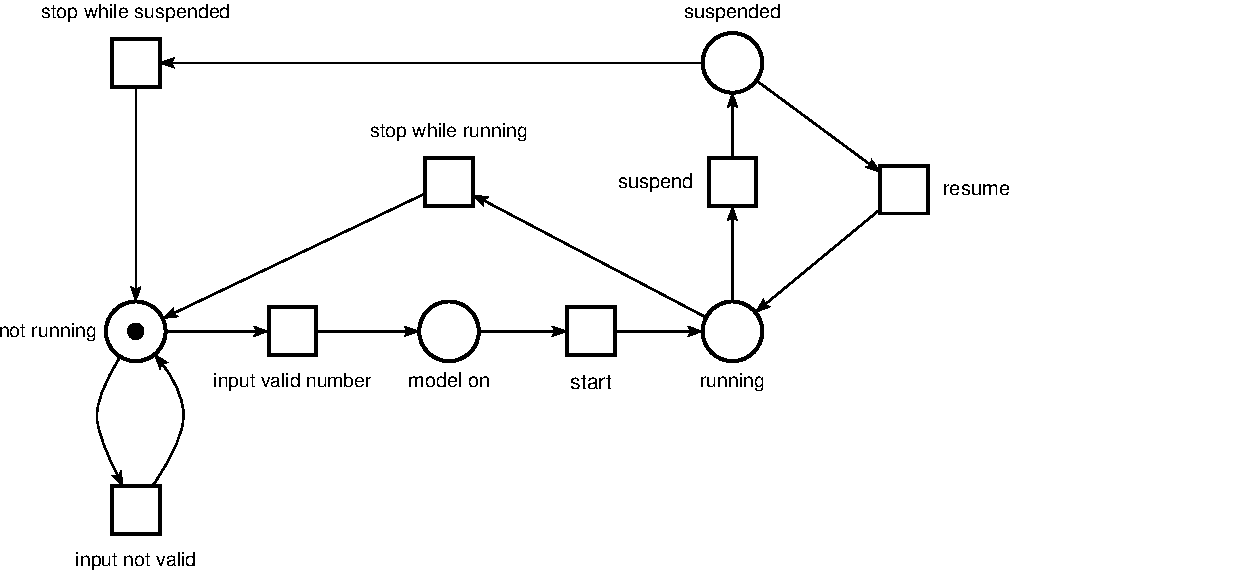
\includegraphics[width=\textwidth]{rete_app_flow.pdf}
    \caption{Rete di Petri per il flusso di esecuzione con input dell'utente.}
    \label{fig:rete_app_flow}
\end{figure}

\section{Ciclo update}
Il ciclo di aggiornamento della simulazione inizia con lo stato iniziale \texttt{start}, seguito dalla fase di calcolo delle velocità (\texttt{update velocity}) eseguita in parallelo da thread distinti (nella figura due). Una volta completato il calcolo, i thread raggiungono una barriera di sincronizzazione (\texttt{velocity barrier}), che garantisce che tutte le velocità siano state aggiornate prima di procedere.

Successivamente, i thread entrano nella fase di aggiornamento delle posizioni (\texttt{update position}), anch'essa eseguita in parallelo. Anche in questo caso, una barriera di sincronizzazione (\texttt{position barrier}) assicura che tutte le posizioni siano state aggiornate correttamente prima di tornare allo stato iniziale, completando così un ciclo di aggiornamento.

Questa rete evidenzia chiaramente i punti di sincronizzazione necessari per mantenere la coerenza del modello, garantendo che le operazioni di calcolo delle velocità e aggiornamento delle posizioni siano eseguite in modo sequenziale e coordinato tra i thread.

\begin{figure}[h!]
    \centering
    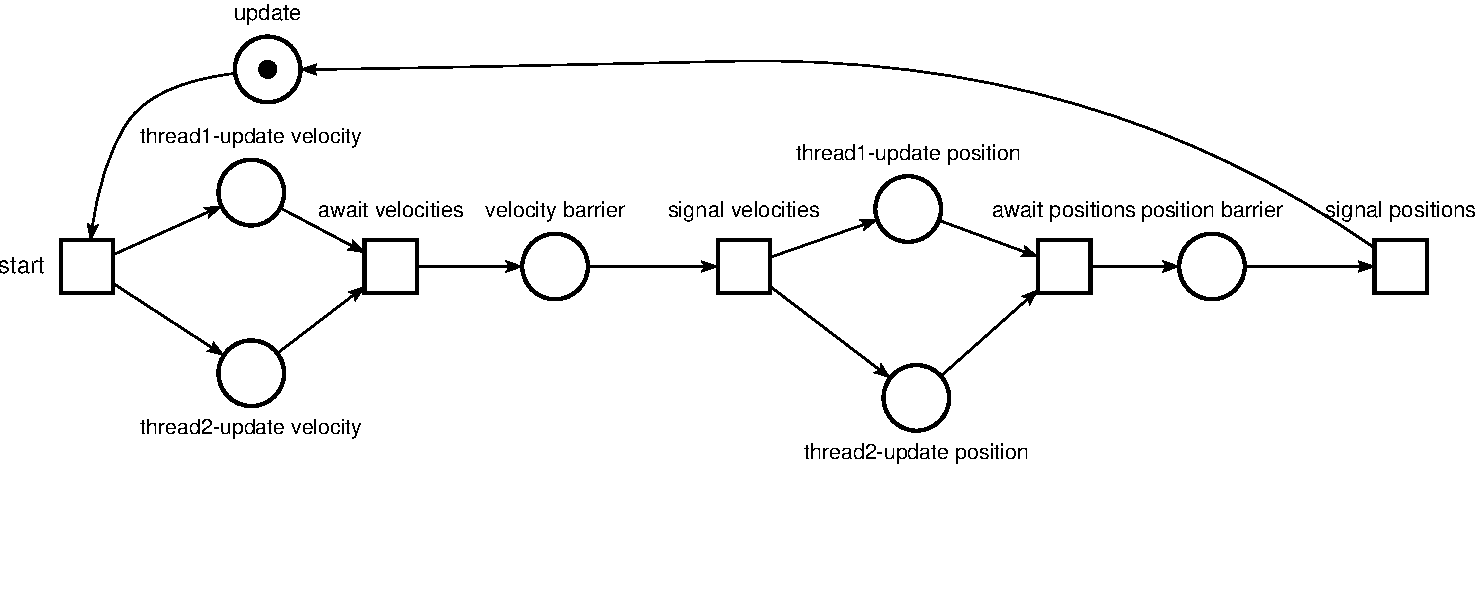
\includegraphics[width=0.8\textwidth]{rete_update_cycle.pdf}
    \caption{Rete di Petri per il ciclo di aggiornamento della simulazione.}
    \label{fig:rete_update_cycle}
\end{figure}

\chapter{Test di performance}
% Performance tests, to analyse and discuss the performance of the programs (for each version) compared to the sequential version
Per valutare l'efficacia delle diverse implementazioni, sono stati condotti test di performance strutturati su diversi scenari e parametri di simulazione. I test sono stati eseguiti su una macchina con [n core] e hanno comparato le quattro versioni dell'algoritmo: sequenziale, platform threads, executor framework e virtual threads.

\section{Metodologia}
I test sono stati condotti con la seguente metodologia:
\begin{itemize}
    \item Numero di boid testati: [range numerico]
    \item Durata di ciascun test: [durata]
    \item Metriche raccolte: framerate medio (FPS)
    \item Numero di ripetizioni per test: [numero] per garantire significatività statistica
\end{itemize}

\section{Risultati}

\subsection{Versione Sequenziale}
\begin{itemize}
    \item Prestazioni baseline con [numero] boid: [valori]
    \item Scalabilità all'aumentare del numero di boid: [descrizione trend]
    \item Considerazioni sul collo di bottiglia: [analisi]
\end{itemize}

\subsection{Versione Platform Threads}
\begin{itemize}
    \item Prestazioni con [numero] boid e [numero] thread: [valori]
    \item Speedup rispetto alla versione sequenziale: [fattore]
    \item Efficienza con diverse dimensioni di partizione: [analisi]
    \item Overhead di sincronizzazione: [valutazione]
\end{itemize}

\subsection{Versione Executor Framework}
\begin{itemize}
    \item Prestazioni con [numero] boid e dimensione task [valore]: [valori]
    \item Speedup rispetto alla versione sequenziale: [fattore]
    \item Impatto della granularità dei task: [analisi]
    \item Overhead di gestione dei task: [valutazione]
\end{itemize}

\subsection{Versione Virtual Threads}
\begin{itemize}
    \item Prestazioni con [numero] boid e [numero] virtual threads: [valori]
    \item Speedup rispetto alla versione sequenziale: [fattore]
    \item Comparazione con platform threads: [analisi differenze]
    \item Comportamento con elevato numero di threads: [osservazioni]
\end{itemize}

\section{Analisi Comparativa}
% Placeholder per un grafico di confronto delle prestazioni
% \begin{figure}[H]
%     \centering
%     \includegraphics[width=0.8\textwidth]{performance_comparison.pdf}
%     \caption{Comparazione del framerate medio tra le quattro implementazioni al variare del numero di boid.}
%     \label{fig:performance_comparison}
% \end{figure}


\chapter{Verifica con JPF}
% Verification of the program (a model of it) using JPF. For this point, only the Java multithreaded programming version may be considered.

\chapter{Esempi di utilizzo}
Esempio di immagine inserita sul posto.
\begin{figure}[h]
\centering{}
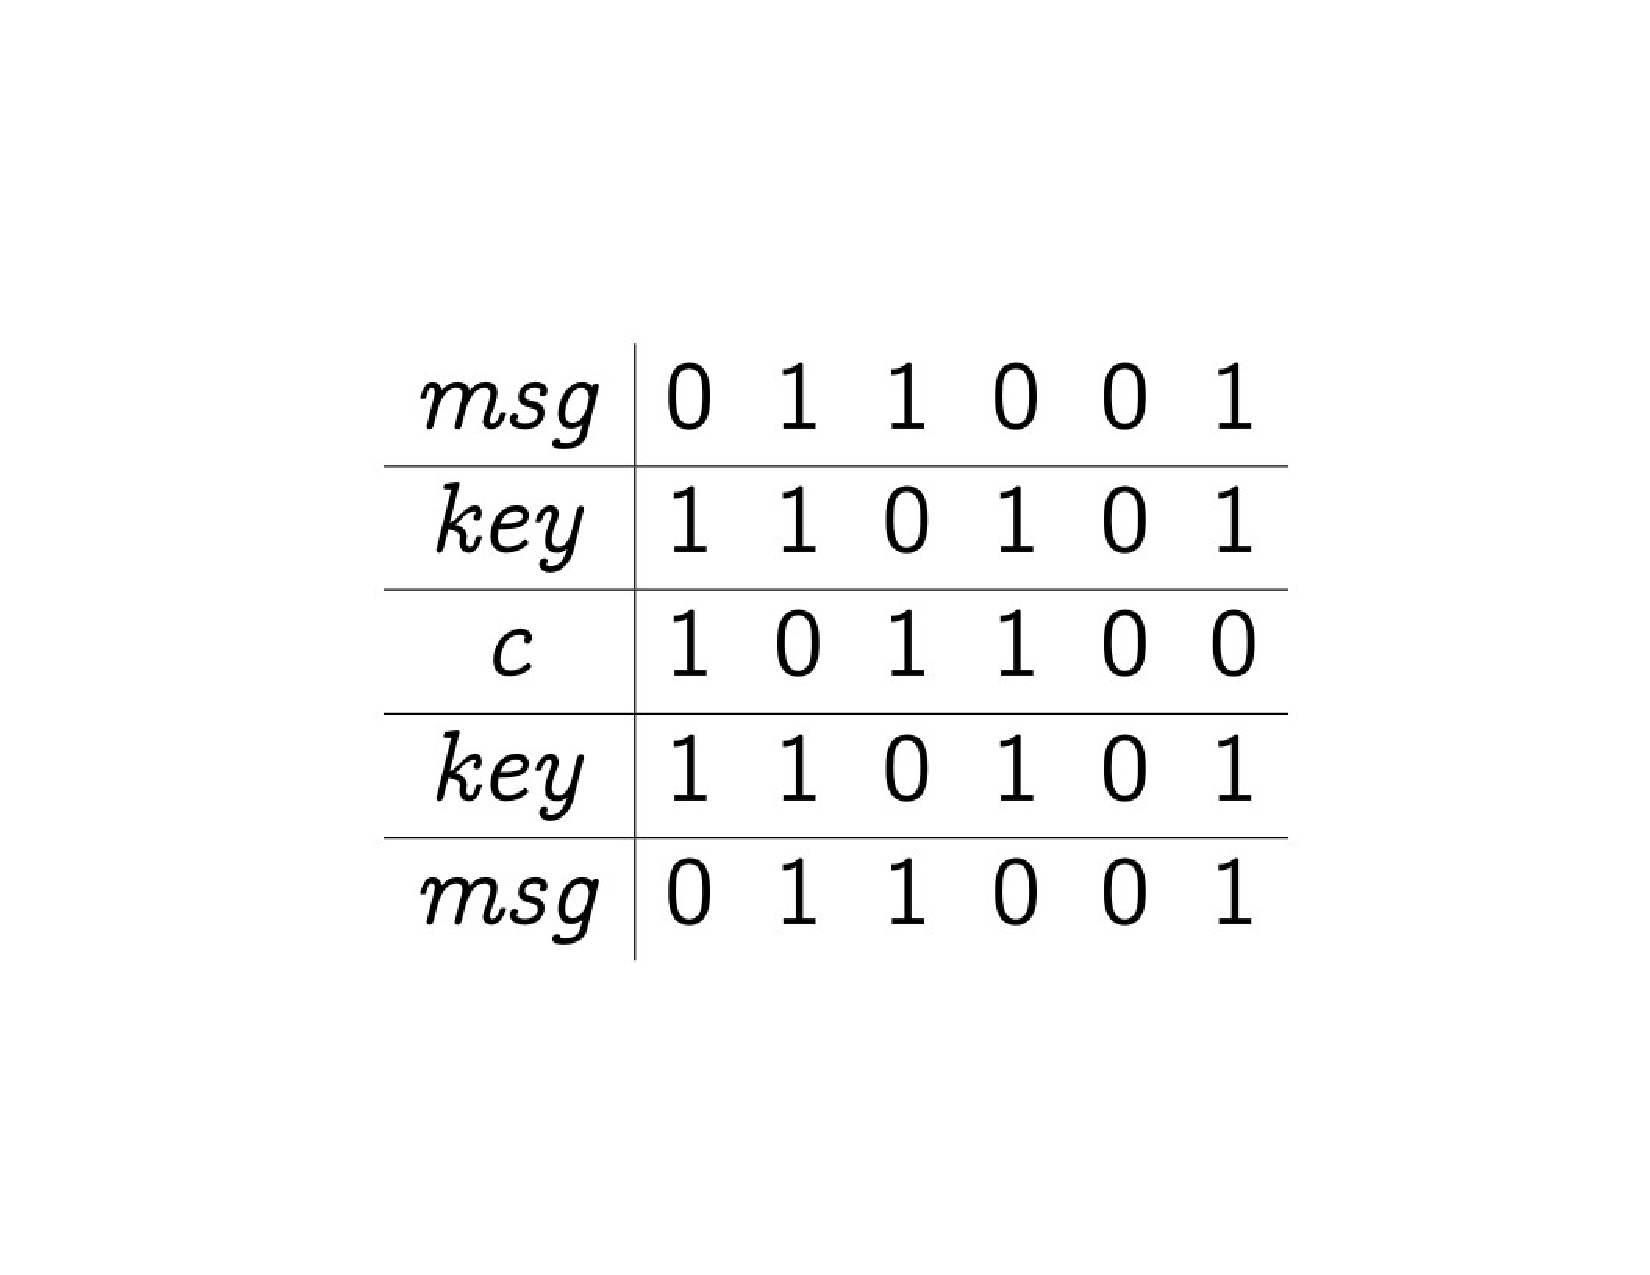
\includegraphics[width=\textwidth]{img/example_img.pdf}
\caption{L'interfaccia \texttt{GLaDOS}.}
\label{img:example}
\end{figure}

\paragraph{Paragrafo Risposta 1} Contenuto \textit{paragrafo}, con riferimento immagine
\Cref{img:example}: e anche \texttt{Scrittura unicode}.

Esempio di link
Permalink: \url{https://github.com/AlchemistSimulator/Alchemist/blob/d8a1799027d7d685569e15316a32e6394632ce71/alchemist-incarnation-protelis/src/main/java/it/unibo/alchemist/protelis/AlchemistExecutionContext.java#L141-L143}

% \appendix
% \chapter{Capitolo appendice 1}

% Contenuto.

% \chapter{Capitolo appendice 2}

% Contenuto.

\bibliographystyle{alpha}
\bibliography{report-template}

\end{document}
